\part{Design, Implementation and Contribution Toward AMAS4Opt}

One of our concerns was not only to propose a new approach for continuous optimization, but also to put this approach in practice by integrating it into a proof-of-concept prototype. To this end we worked with domain specialists and software development experts to propose such a tool, basing ourselves upon the ADELFE method. This method aims to guide the development of AMAS-based softwares from high level user requirements to the implementation nuts and bolts. Using ADELFE we made a formal analysis of the domain and actor involved in the use of such tool.

We also use the design tools developed in conjunction with the method to instantiate our MAS with the final end to integrate it with a functional end-user interface. Notably, the recent MAY framework, which was developed in order to provide suitable abstractions as well as reusable software components for the development of agents and multi-agents systems. We contributed to the enrichment of its component library by developing a a general and modular agent architecture consistent with the AMAS theory, in particular by proposing a modular skill stack principle, where different skills can be composed to address specific requirements.

While such work could seems to concerns more software engineering experts than computer scientists, we will see how existing MAS oriented methods such as ADELFE are still too broad level to be successfully directly applied to any domain (and more so to continuous optimization) without an important agent expertise and extensive research work. We will detail how the scientific work we produced and presented in the previous part, especially the identification of various NCS and the mechanisms to solve them, can be generalized into \enquotes{building blocks}. These building blocks could be then reused to guide the conception of other MAS for the domain of problem solving. This work places itself into a more general effort to provide a general reusable toolbox for assisting non experts in applying AMAS to the domain of optimization, under the name \emph{AMAS4Opt} (AMAS for Optimization).

\chapter{ADELFE}

\section{Overview of ADELFE}

In section \ref{AMAS-ADELFE}, we succinctly presented ADELFE, the method which has been proposed for the design of AMAS. In this chapter we get back in more details about this method and what benefits it provided for the design of our system. 

The ADELFE method in itself is based the Rational Unifed Process (RUP) and is defined following the Software Process Engineering Meta-Model (SPEM)  \cite{bernon2003adelfe,picard04phdthesis}. Since its revision \cite{Ro2008.3}, it is composed of five \emph{Work Definitions} ($WD$), themselves decomposed in several \emph{activities} making use of UML as well as the AMAS-ML and muADL languages. An overview of the method is shown on \figurename{} \ref{ADELFE_phases}.

\begin{figure}
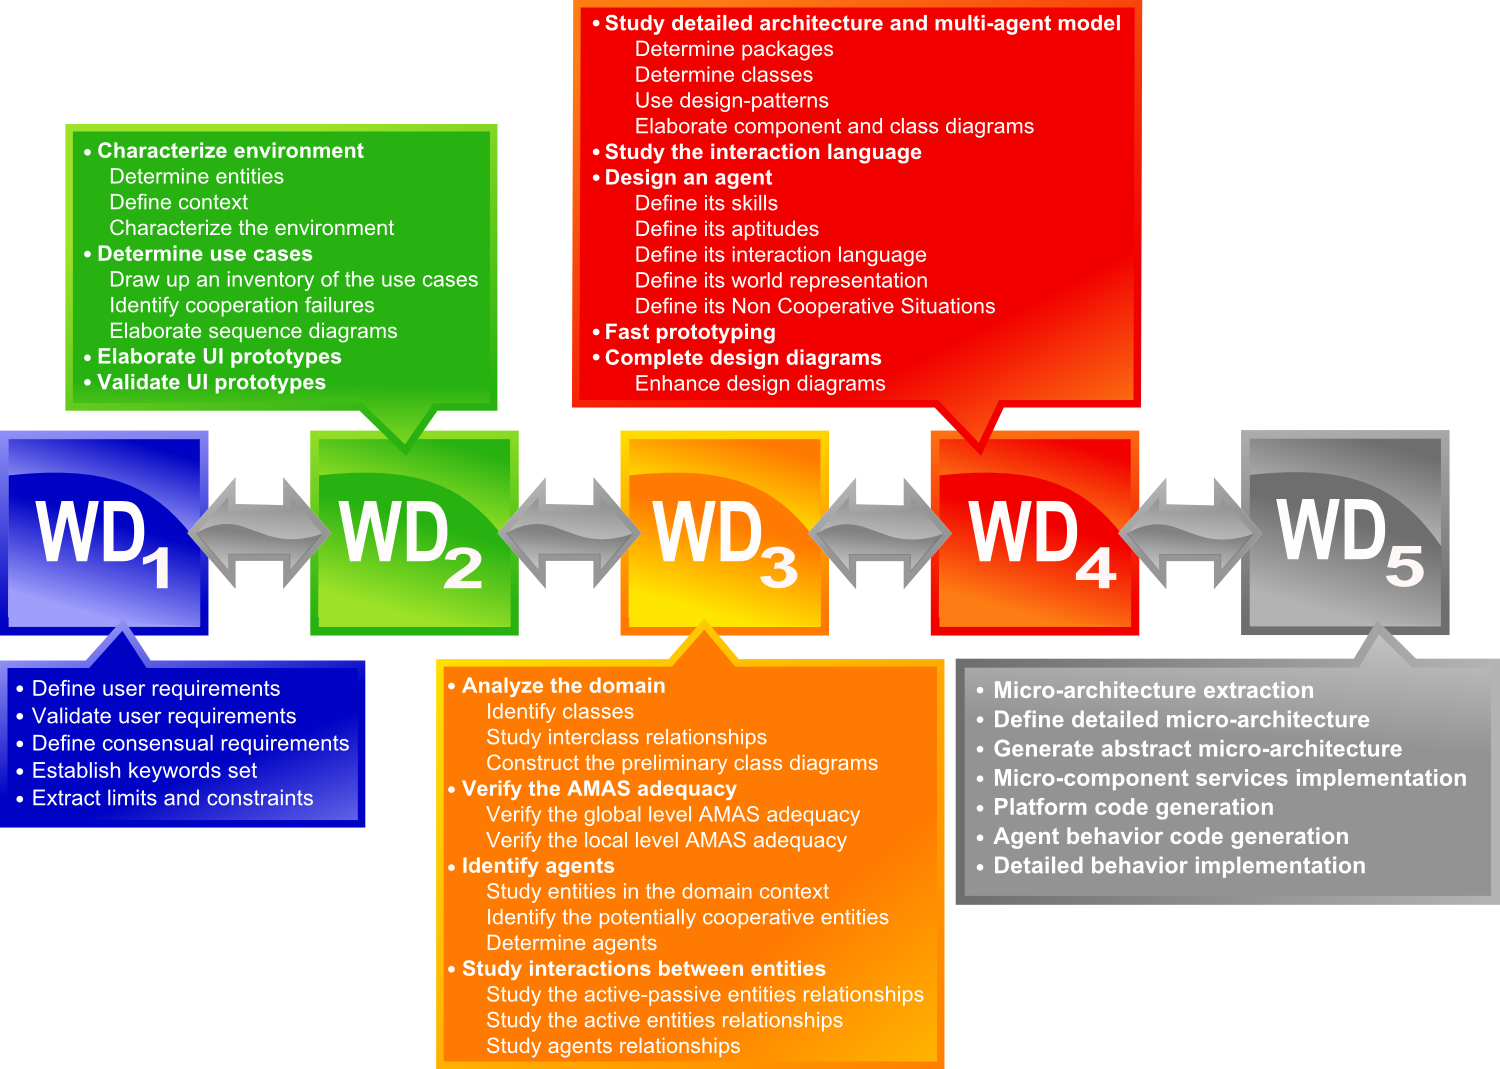
\includegraphics[width=\textwidth]{AdelfePhases}
\caption{Overview of the ADELFE Method}\label{ADELFE_phases}
\end{figure}

In regard of the RUP, ADELFE adds specific activities and roles which are specific to its approach for the design of AMAS.\\
The final requirement study ($WD_2$), was complemented with activities 6 and 7-2 concerning the characterization of the system environment and the identification of cooperation failures during the determining of the use cases.During the Analysis ($WD_3$), additional activities 11 and 12 respectively check for the adequacy of AMAS to the problem and identify the agents involved in the system being built, while activity 13 is complemented with a step concerning the study of the relationships between agents. During the design ($WD_4$), activities 15 et 16 concerns the design of the system and the agents, while activity 17 concerning fast prototyping was added in order to be able to quickly test the proposed behavior of the agents. The development phase ($WD5$), which was not present in the initial version of ADELFE, concerns the architecture and the implementation of the agents and the system.

\section{Applying ADELFE for the Design of a Continuous Optimization Tool}

\begin{figure}
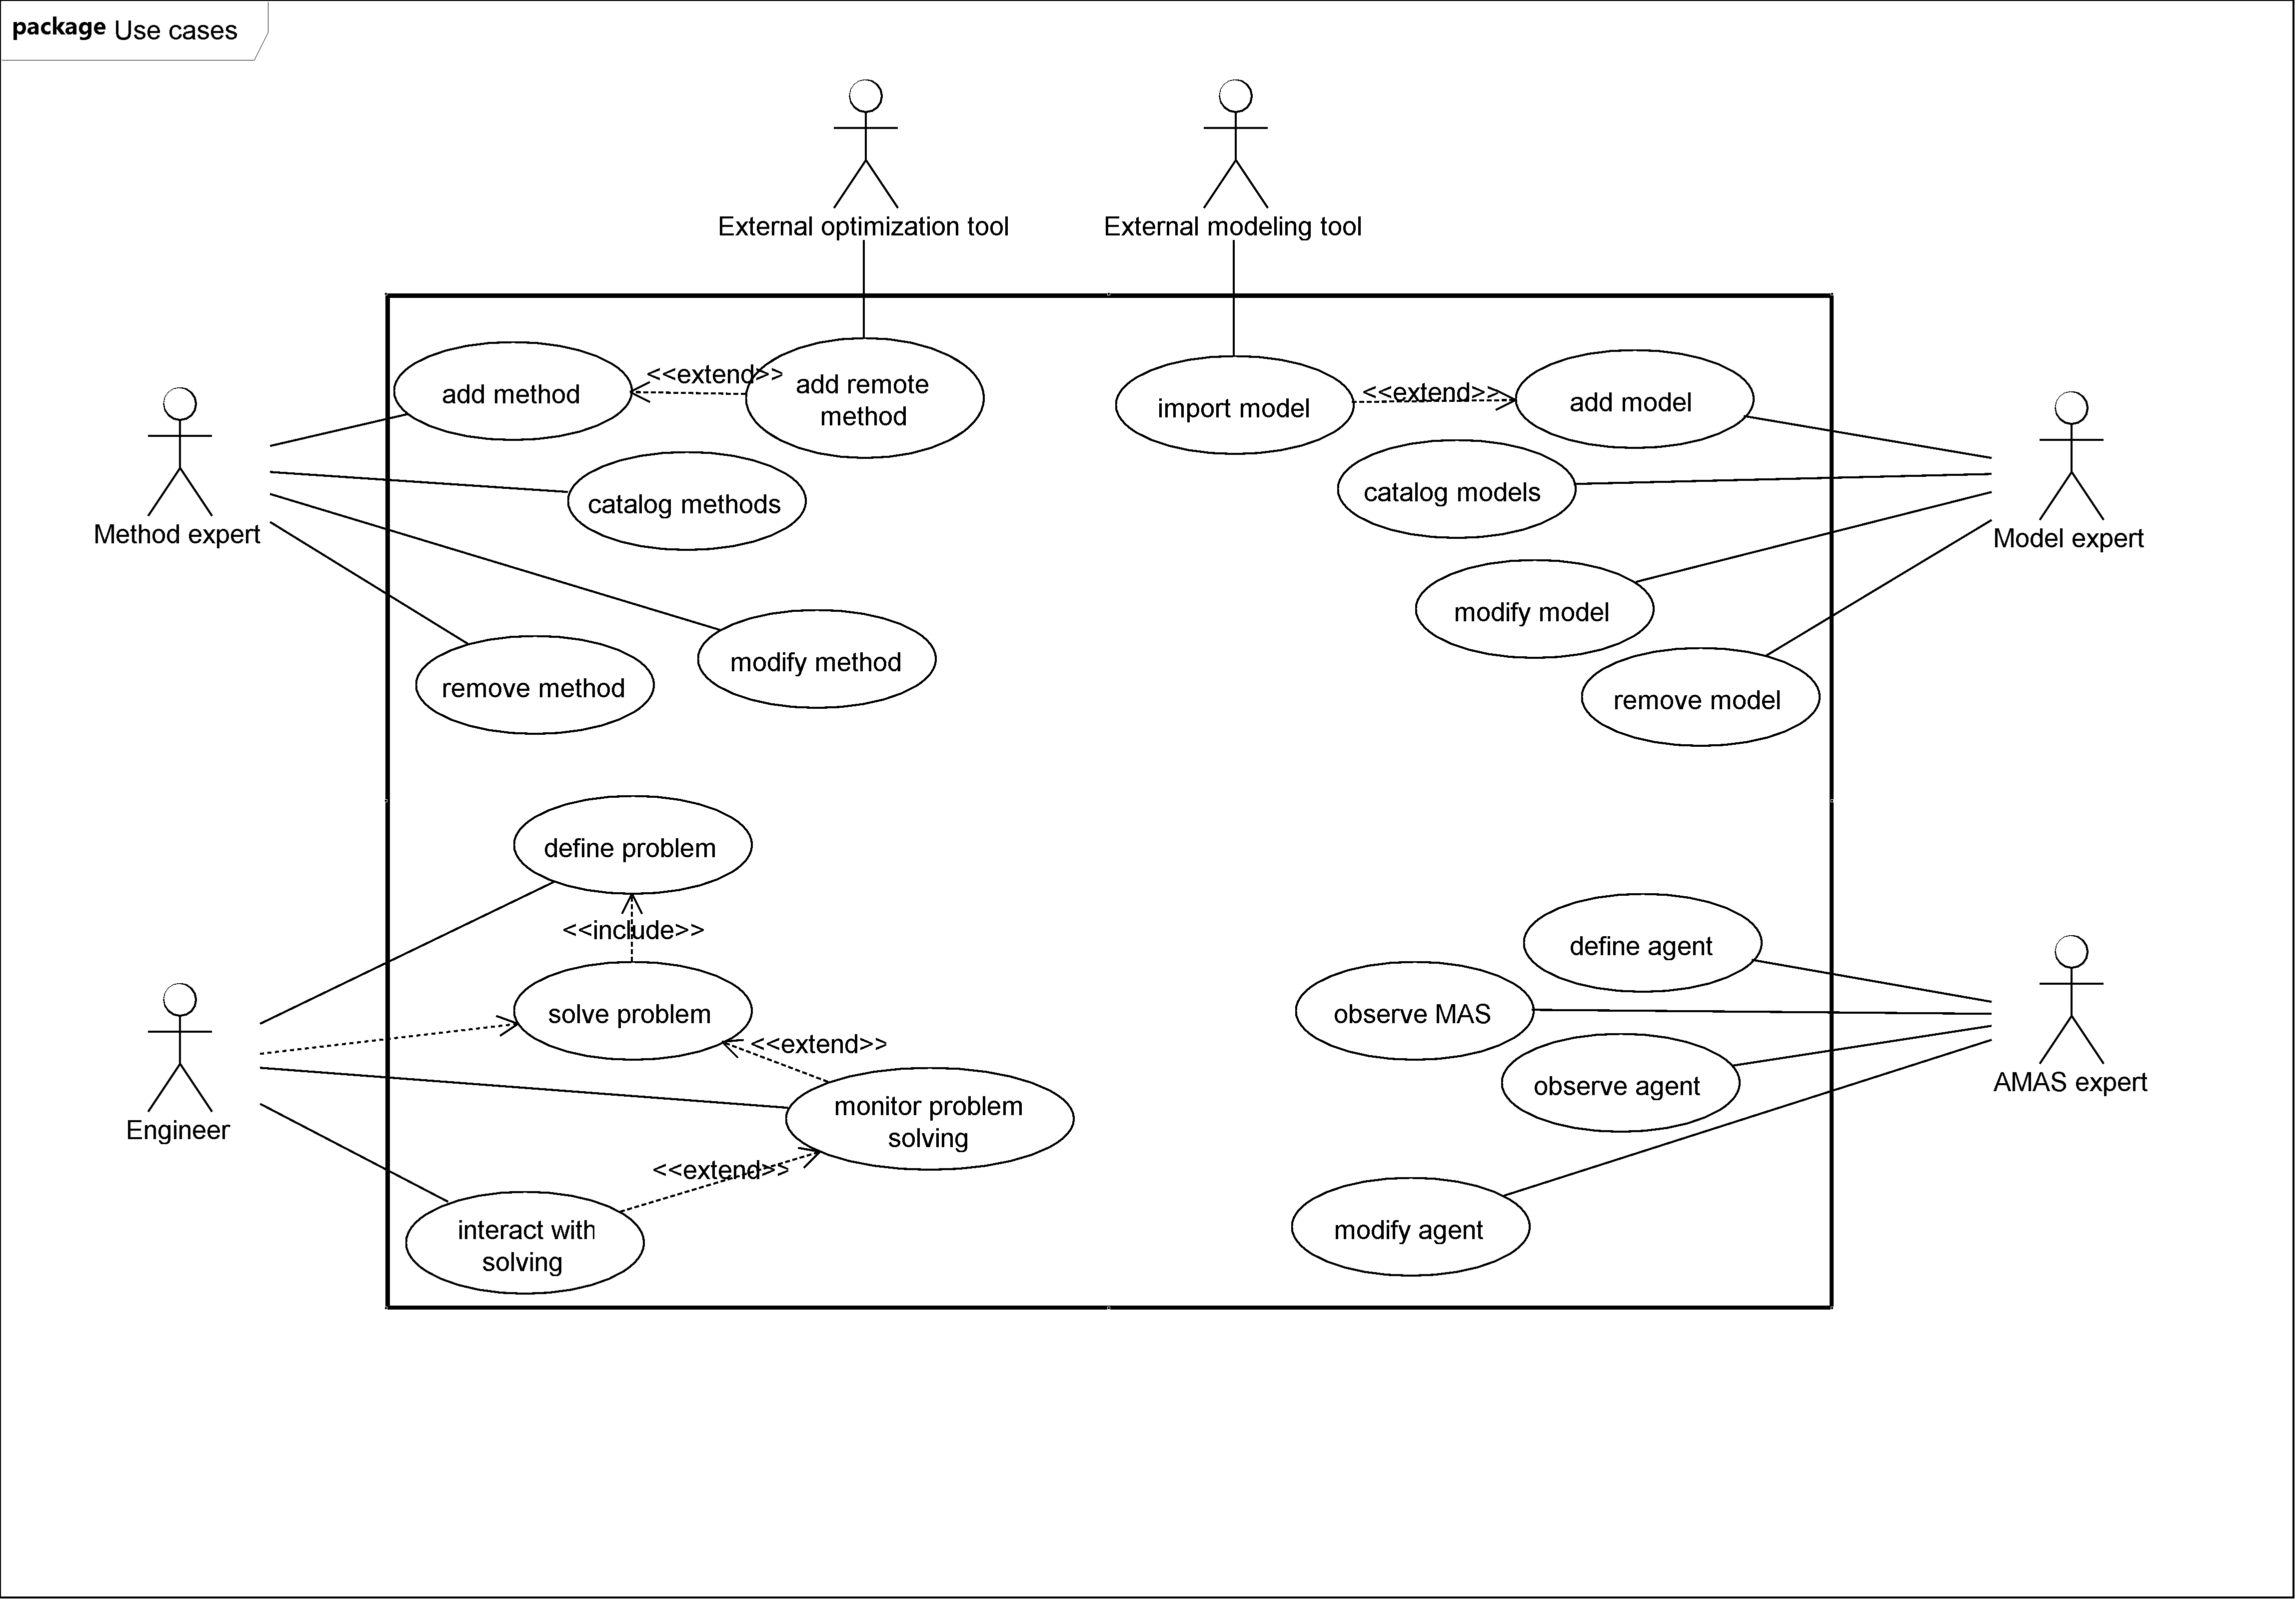
\includegraphics[width= \textwidth]{Use_cases}
\caption{Actors and use cases identified during requirements studies}
\end{figure}


\chapter{MAY Architecture}

[[First generic AMAS architecture ??]]

To implement the MAS, we used the Make Agents Yourself (MAY) framework. MAY is a component-based framework which automatically generate an implementation of an agent architecture from a given description.

[[PROVIDE SOME REF -> ASK VICTOR -> his phd \cite{No2012.2}]]

The Adelfe methodology proposes an abstract agent architecture (represented in \fig{[[TODO]]}), which we translated into the MAY architecture description language, SpeADL. [[As our agents only act and communicate using message-passing, we could make some simplification concerning the modeling of the communication and action capabilities.]]
All our agents use the same AMAS architecture. They are differentiated by specific implementations of the components. For example, \emph{Model} and \emph{Variable} agents will have different implementations of the \emph{Behavior} component.

For the sake of clarity, the agent architecture is separated in three views: the \emph{behavior}, \emph{communication} and \emph{monitoring} views.

\subsection{Behavior}

The \emph{behavior} view (\figurename{} \ref{Arch-behavior}) contains the components related to the behavior of the agent. 

\begin{figure}
\centering
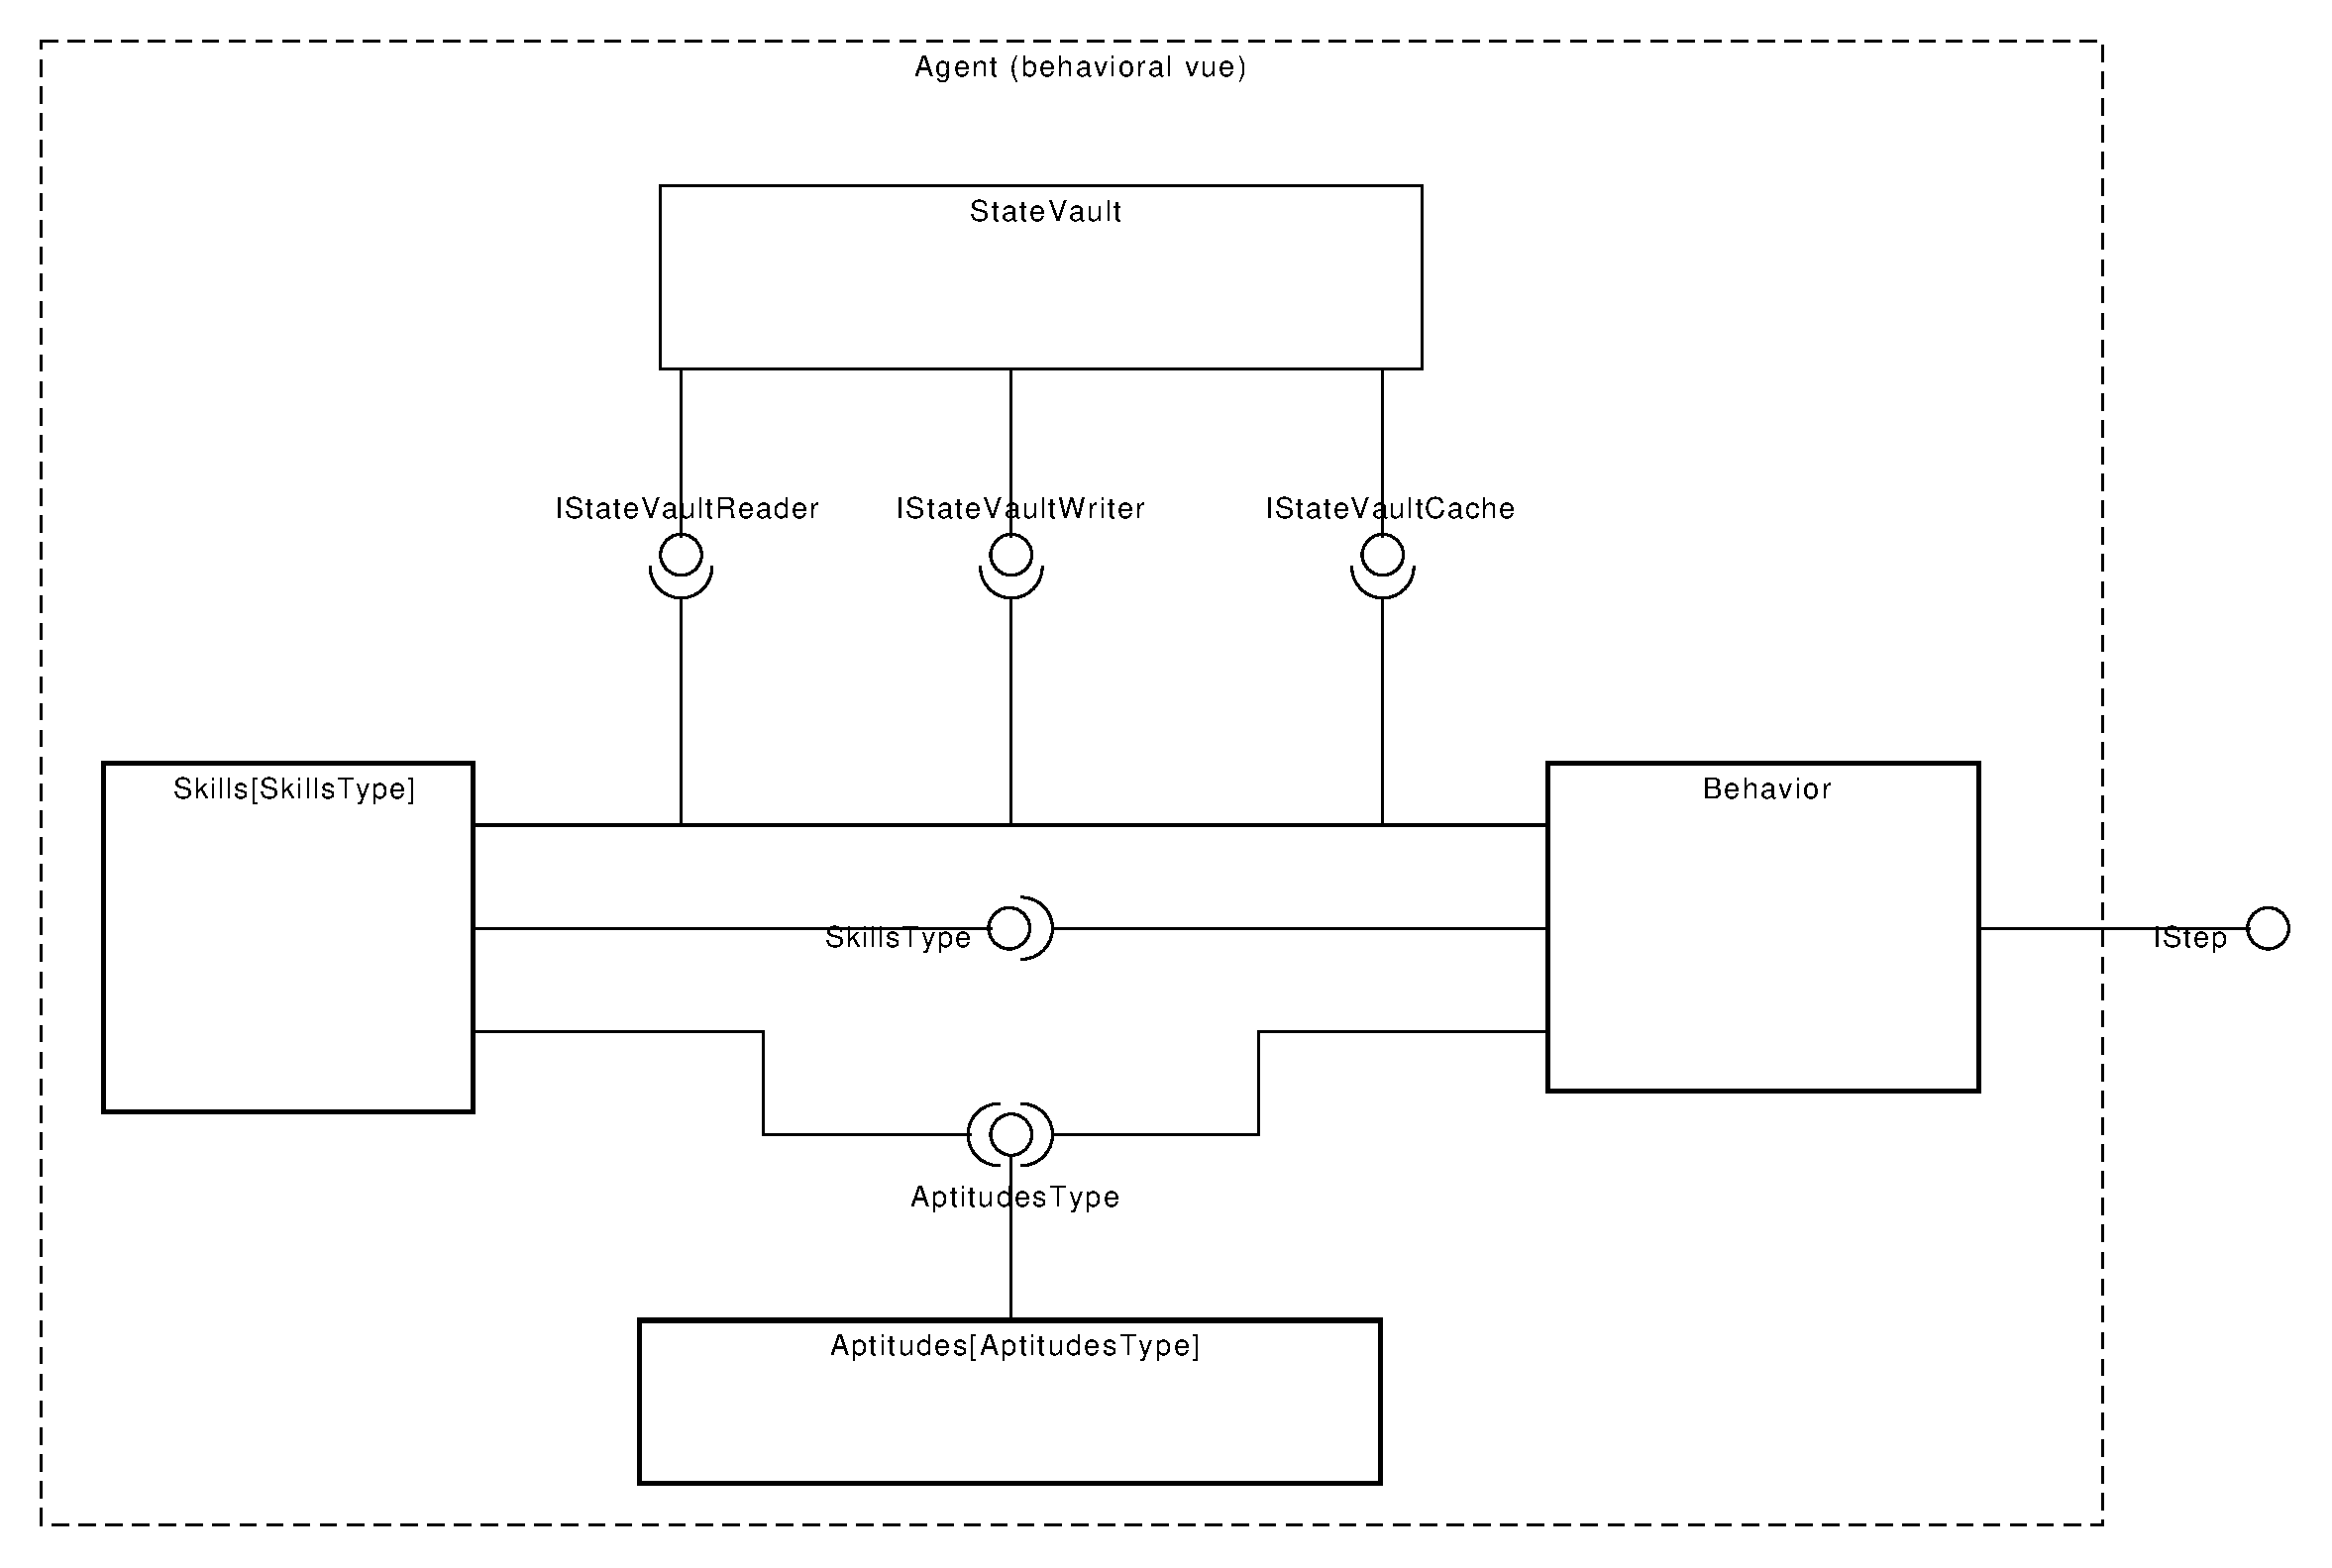
\includegraphics[width=0.6\paperwidth]{ID4CS_Speadl_behav}
\caption{Agent Architecture - Behavior view.}
\label{Arch-behavior}
\end{figure}

The \emph{Behavior} component contains the rules which dictate the behavior of the agent. This component can be seen as the [[chef d'orchestre]] of the architecture. This component exposes to the outside of the environment the \emph{Step} port, which is used to make the agent execute a step. During a step the \emph{Behavior} component executes the agent rules. These rules will in return make use of the others components of the agent.

[[DIRE QUE LES RULES ONT ETE PRESENTEES DANS UN CHAPITRE PRECEDENT]]

The \emph{State Vault} contains the state of the agent. It is used by the components which need to save and read some state variables. Centralizing all the states variables into one component provides several benefits. First it is easier to save and restore the state of the agent, as we just need to save the content of the vault. It is also simple to share some data between components, as long as these components have access to the vault. And it is easy to provide a view of the agent state by just reading the State Vault.
This approach has however several drawbacks. It adds some boilerplate code when writing code using the agent state, as we need to explicitly read the value from the vault (and possibly store it to the vault if modified). It make more difficult to track side-effects, as it is not obvious to know which component uses which value. At last there is no way to strictly enforce that components only use the State Vault for storing state values, as neither Java nor MAY can provide such guarantee.

The \emph{Skills} component contains the skills of the agents. Skills are [[skill definition]]. Each agent type has its own skills set, and skills can require to read and modify the agent state (thus the link between this component and the \emph{State Vault}).
Some skills are used directly from the \emph{Behavior} rules but some skills can also be used by others skills.
Some examples of skills are: for a \emph{Variable agent}, the capability to change its value based on the requests it received and its old value. For a model agent, the capability to translate a request it received to change one of its outputs into a set of requests to send to its inputs.

[[PARLER DU FAIT QUE LES SKILLS ONT LEUR PROPRE ARCHITECTURE ??]]

The \emph{Aptitudes} component contains the aptitudes accessible to the agents. Aptitudes are [[Aptitude definition]]. Unlike skills, aptitudes are general capabilities which do not rely on the state of the agent. Consequently, all agent types have access to the same aptitudes, and there is only one implementation of the \emph{Aptitudes} component.
Some aptitudes are used directly from the \emph{Behavior} rules but some aptitudes can also be used by skills or others aptitudes.
Some examples of aptitudes are: ordering a set of requests from the most to the least important. Make some manipulations on the exchanged values (adding, calculate the norm etc.).

\subsection{Communication}

The \emph{communication} view (\figurename{} \ref{Arch-comm}) presents the components related to the communication capabilities of the agent. 

\begin{figure}
\centering
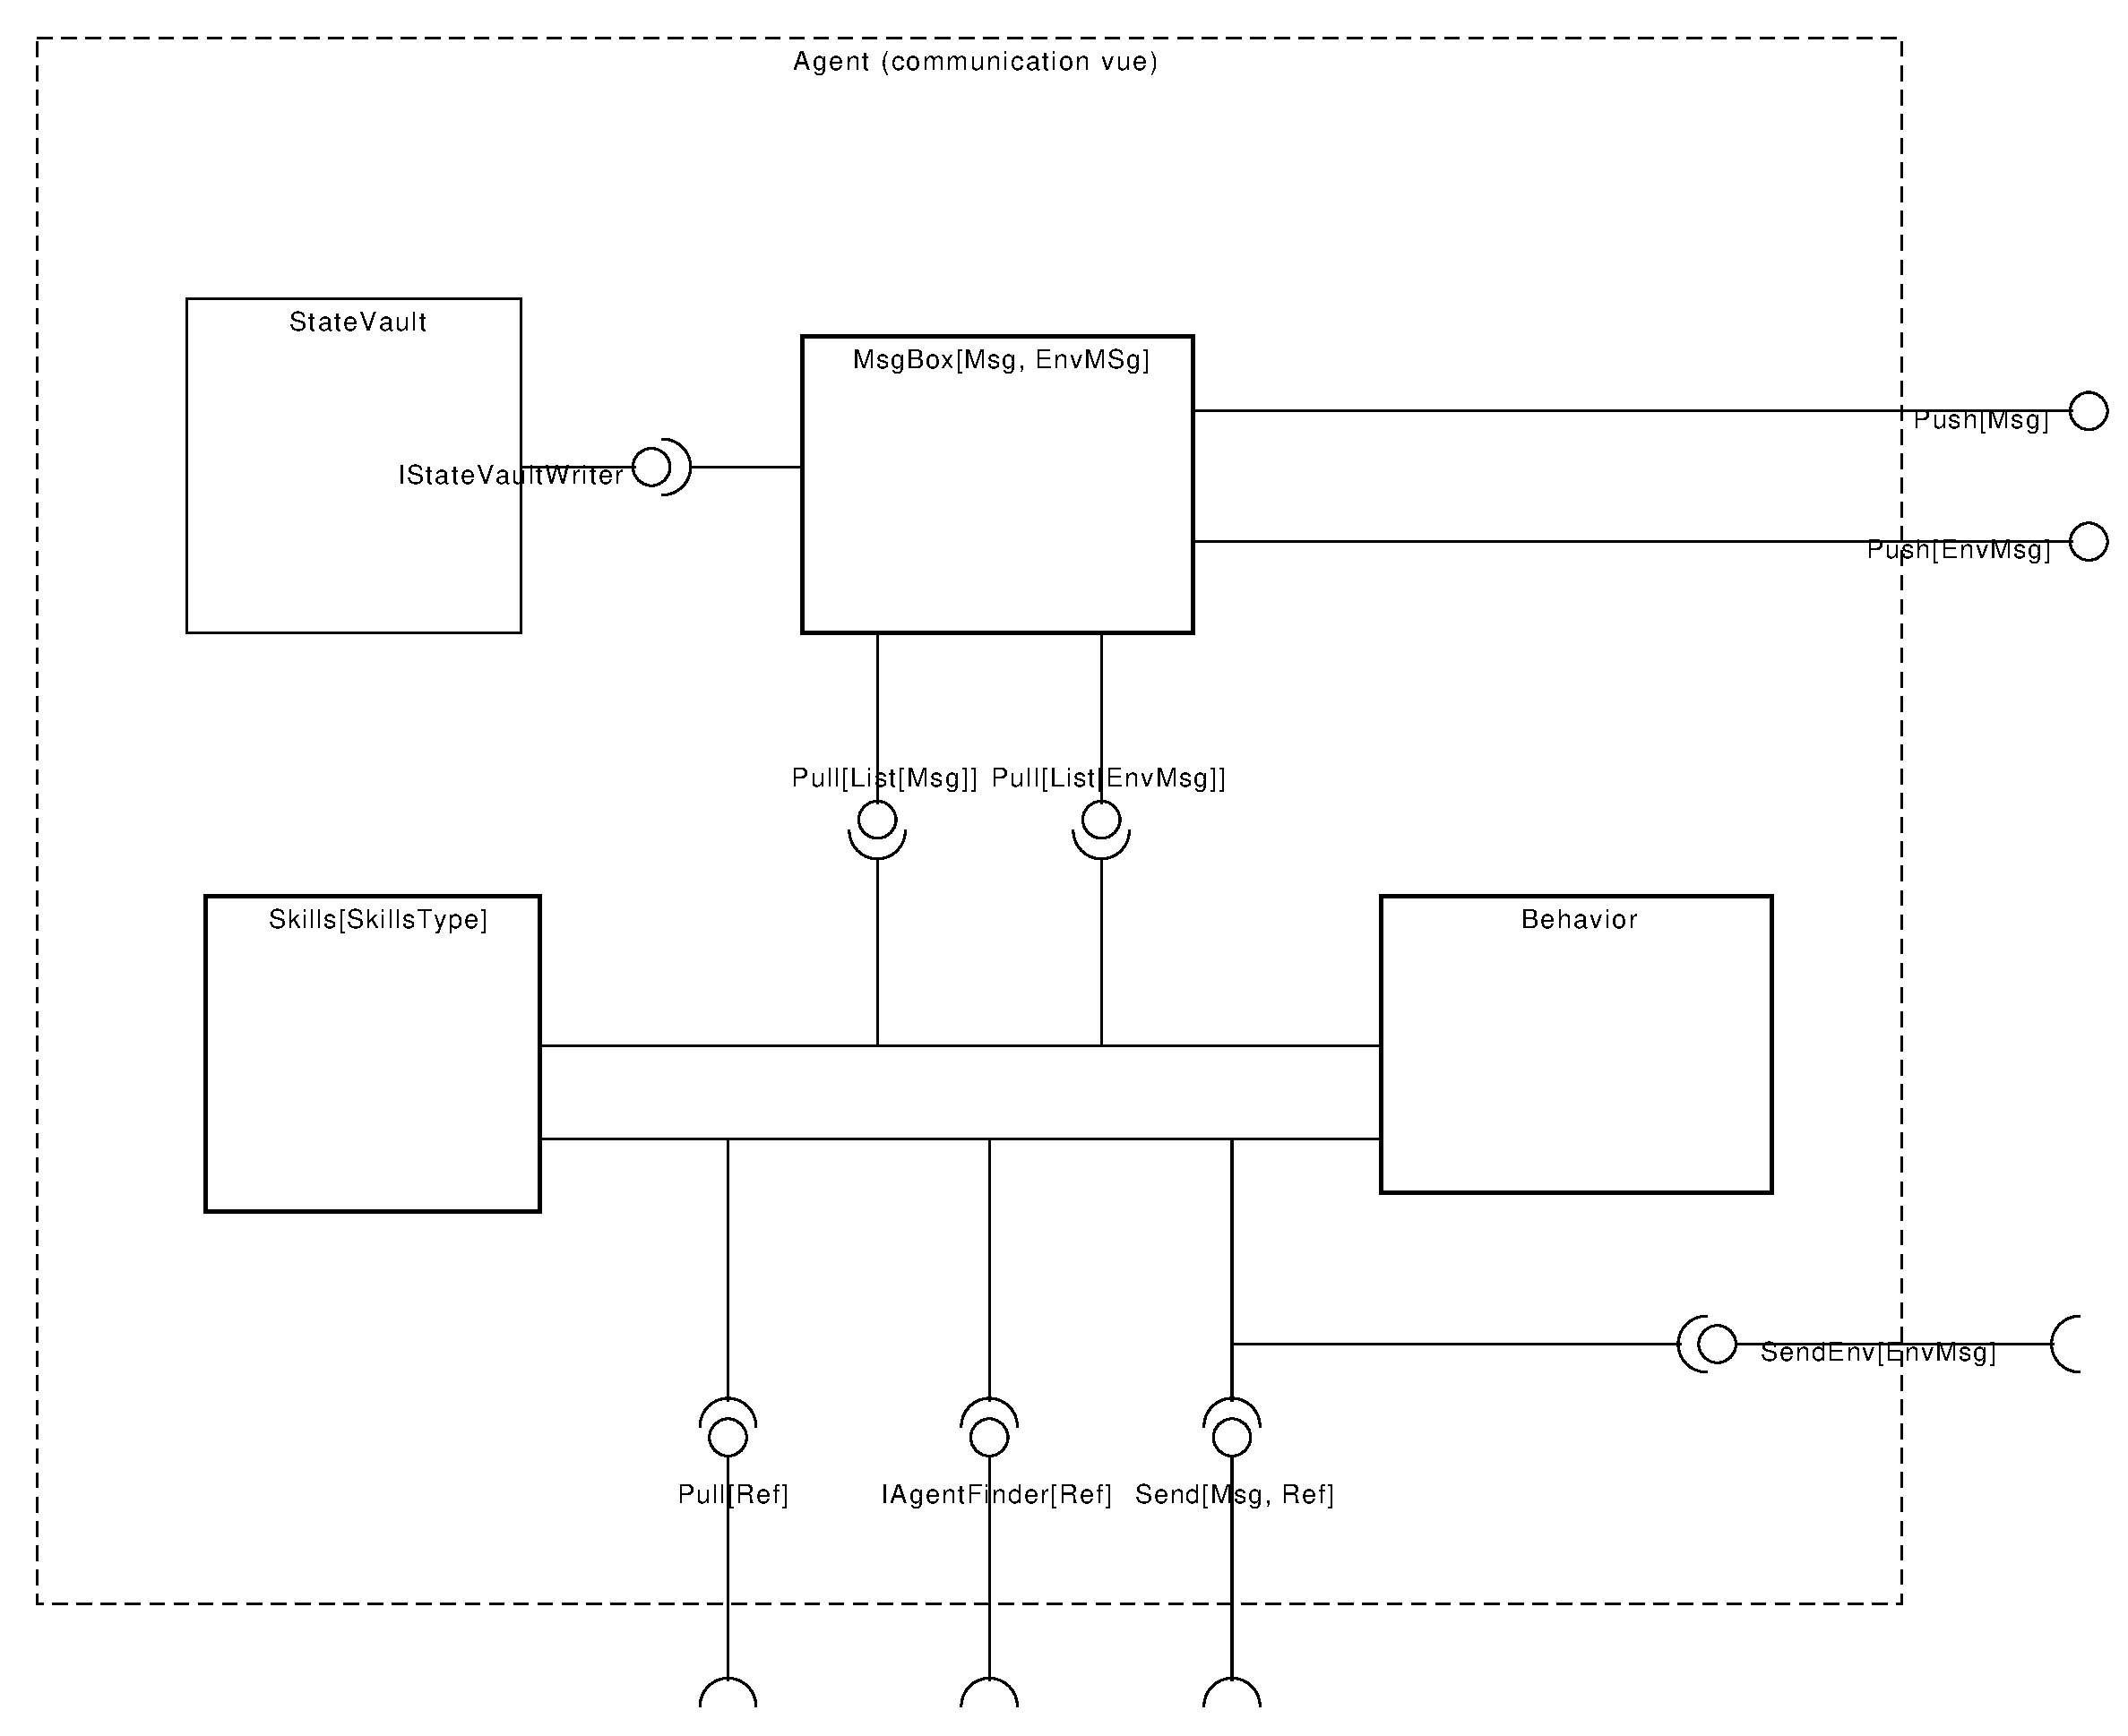
\includegraphics[width=0.6\paperwidth]{ID4CS_Speadl_comm}
\caption{Agent Architecture - Communication view.}
\label{Arch-comm}
\end{figure}

This view contains the new component \emph{Message Box}, which contains the messages sent to the agent. The \emph{Message Box} stores the messages into the \emph{State Vault} and provides a direct access to the \emph{Skills} and {Behavior} components.

This figure presents several ports which need to be provided from the environment to the agent. The environment must give an unique \emph{Reference} to the agent, which will be used by the others agent to communicate with it. The environment must also provides some ports to communicate with the others agents and outside of the system.
[[PARLER DE L'AGENT FINDER ??]]

\subsection{Monitoring}

The \emph{monitoring} view (\figurename{} \ref{Arch-monitor}) presents the components related to the monitoring of the agent. 

The new component introduced in this view is the \emph{Monitor}. The \emph{Monitor} provides to the environment to ports. The first port is used for external monitoring interfaces to subscribe to be informed of changes in the state of the agent. The second is used to provide informations concerning changes of a specific part of the agent. Thus, an external monitoring interface can subscribe to be notified when the state of the agent changed using the first port, and then use the second port to access to the specific informations it want to monitor.

In order to provide its capabilities, the monitor agent need to be informed by the \emph{Behavior} component before and after each step, to read and compare the monitored informations into the \emph{State Vault}.

\begin{figure}
\centering
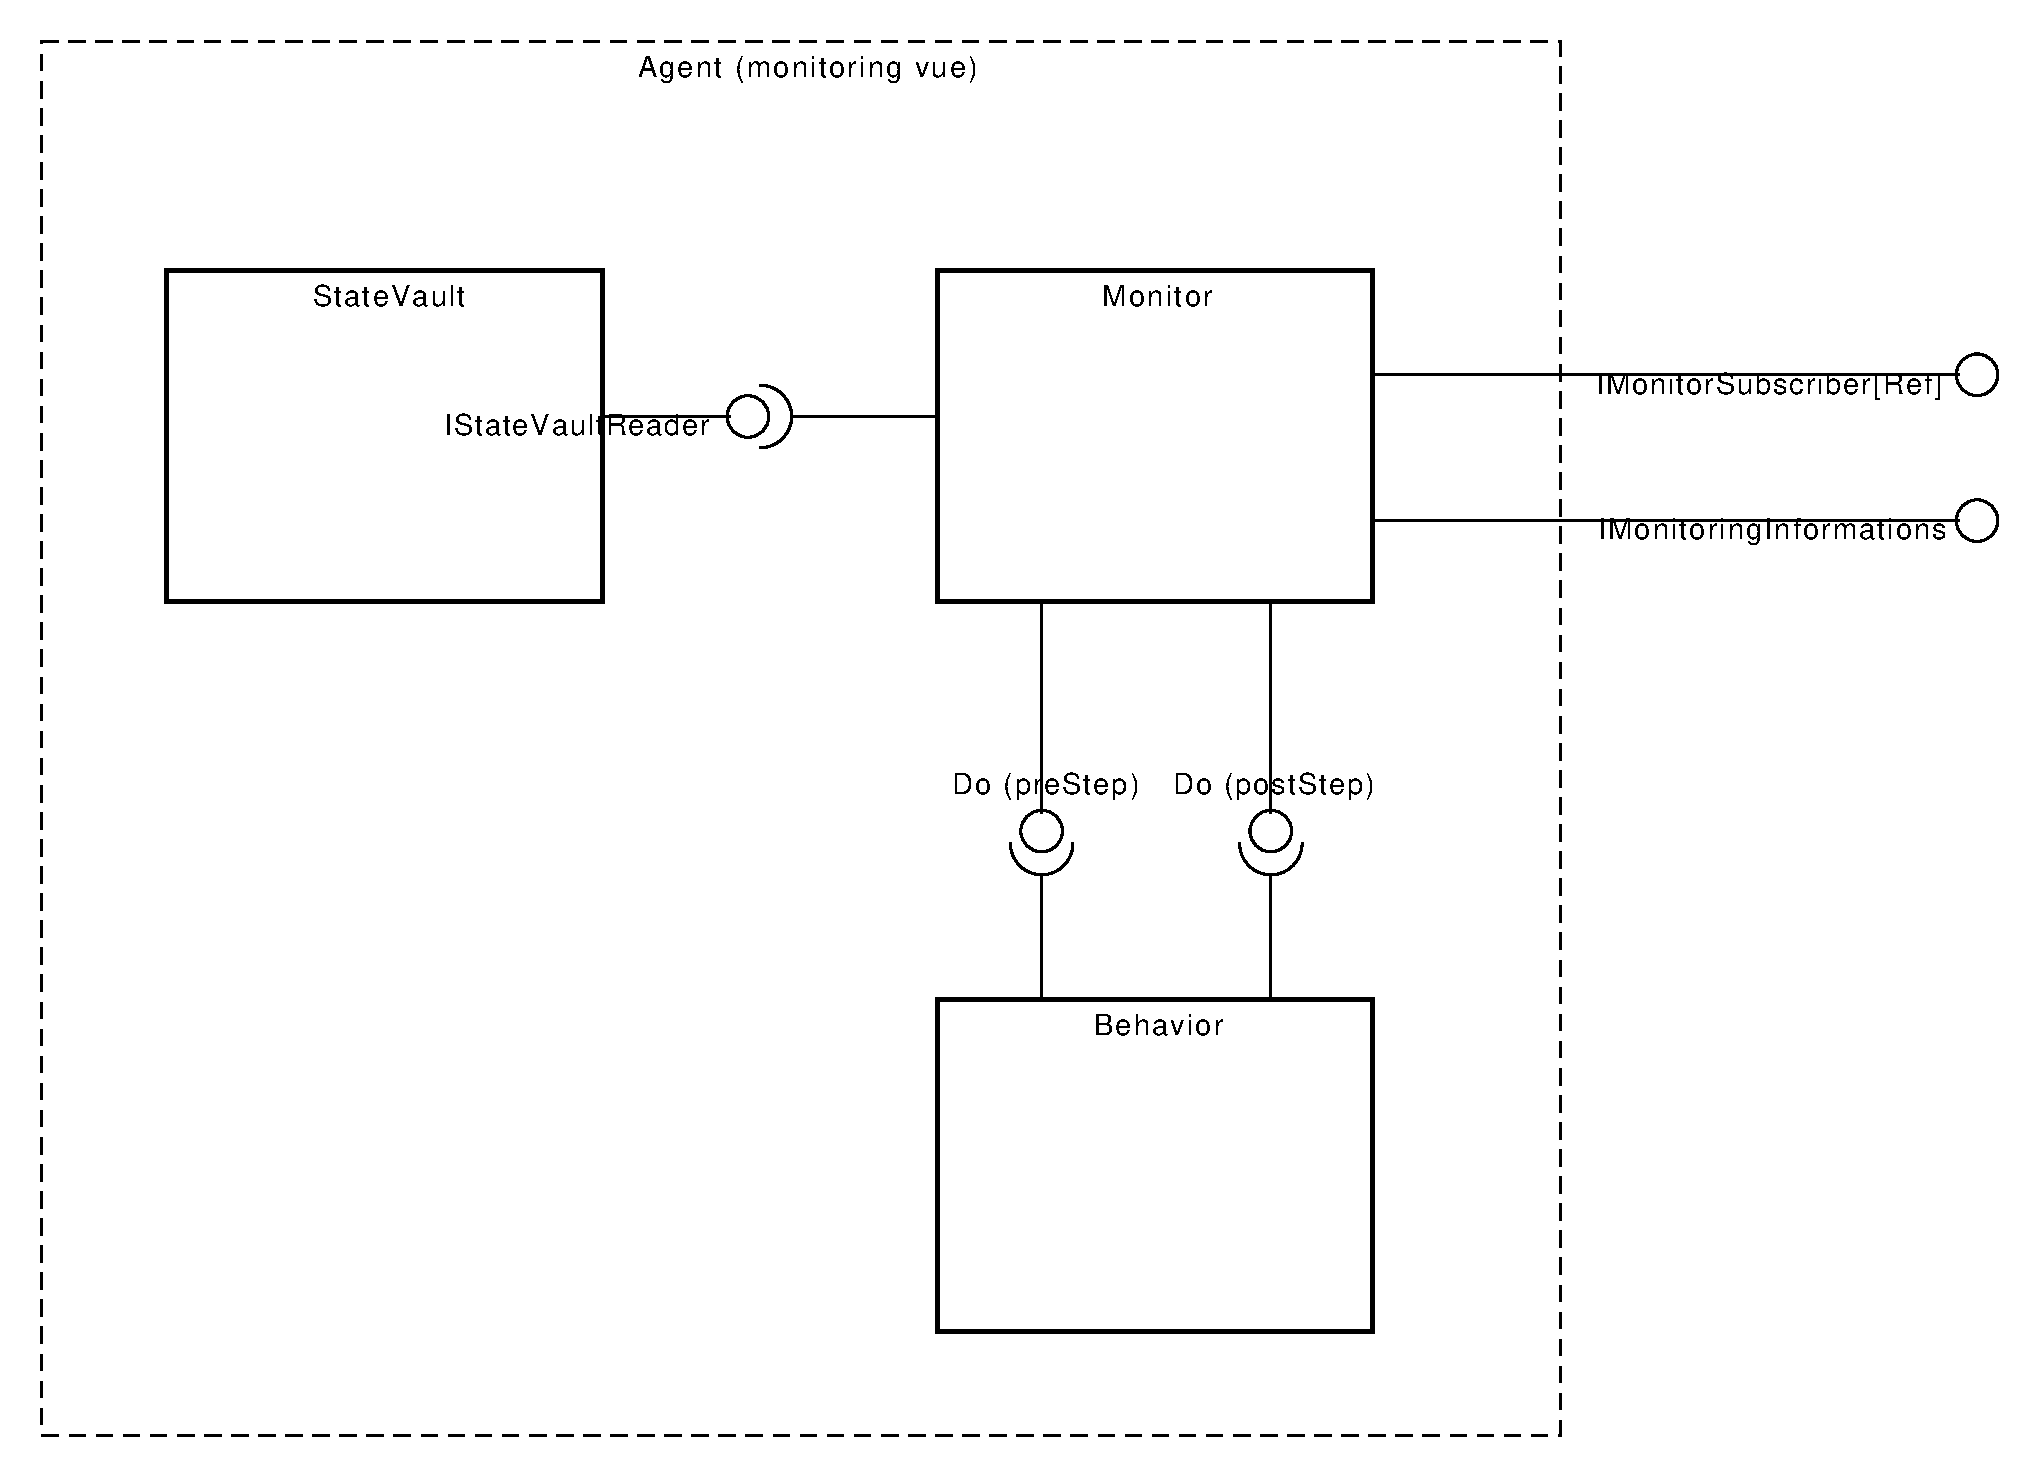
\includegraphics[width=0.6\paperwidth]{ID4CS_Speadl_monitoring}
\caption{Agent Architecture - Monitoring view.}
\label{Arch-monitor}
\end{figure}

\section{MAS Architecture}

\section{Integration into the prototype}

[[OSGI and EMF]]

This implementation of the MAS was part of a collective development effort to provide a functional prototype. The goal of this prototype is to be a proof-of-concept tool of the possibilities offered by agent-based continuous optimization.

The development of the prototype was carried mainly by three partners[[cite them?]], each in charge of a different aspect.

The prototype can be divided in three parts: The Graphical User Interface (GUI), the core module (CORE) and the Multi-Agent Système (MAS). The CORE provides a common representation of the manipulated data and is in charge of maintaining consistency between the GUI and the MAS.

These three modules communicate using the OSGi framework\footnote{\url{http://www.osgi.org}}.

\subsection{MAS}

We already presented the implementation of the MAS in the previous parts. The only additional work was to encapsulate the implementation into an OSGi [[service]].

\subsection{CORE}

The CORE module is responsible of maintaining consistency of the manipulated data. It serves as a middle-man between the MAS and the GUI.

[[Insert full Data Model and comment]]

\subsection{GUI}

The GUI was build using the [[Eclipse Framework]].


